%% Template baseado no do Prof. Arnaldo Mandel
%% Veja https://www.ime.usp.br/~am/414/listas/index.html

\documentclass[12pt]{article}

%% Escrevendo em português:

%\usepackage[brazilian]{babel}
\usepackage[utf8]{inputenc}
%\usepackage{textcomp}
\usepackage[T1]{fontenc}
\usepackage{lmodern}
%----------------------------

\setlength{\topmargin}{-.5in}
\setlength{\textheight}{9in}
\setlength{\textwidth}{6.3in}
\setlength{\oddsidemargin}{-.125in}
\setlength{\evensidemargin}{-.125in}

\usepackage[usestackEOL]{stackengine}
\usepackage{xspace}
\usepackage{pifont}
\usepackage{amsmath}
\usepackage{amsfonts}
\usepackage[dvipsnames]{xcolor}
\usepackage{fancybox}
\usepackage{amsthm}
\usepackage{listings}
\usepackage{hyperref}
\usepackage{todonotes}

\usepackage{MnSymbol,wasysym}
\usepackage{marvosym}

\pagestyle{empty}

\definecolor{darkgreen}{RGB}{0, 133, 117}
\definecolor{yelloworange}{HTML}{FAA21A}

\newcommand{\N}{{\tt I\kern-.2em N \relax}}      % N        |N
\def\pule{\vspace{0.2cm}}
\def\pulao{\vspace{0.5cm}}
\def\pulaozao{\vspace{1cm}}
\def\ni{\noindent}

\newcommand{\Si}{\ensuremath{\Sigma}\xspace}
\newcommand{\Sis}{\ensuremath{\Sigma^*}\xspace}
\newcommand{\Ga}{\ensuremath{\Gamma}\xspace}
\newcommand{\Gas}{\ensuremath{\Gamma^*}\xspace}
\newcommand{\serio}{\ding{98}\xspace}
\newcommand{\LP}{L\&P\xspace}
\newcommand{\conj}[2]{\ensuremath{\{#1\,|\;#2\}}}
\DeclareMathOperator{\Ima}{Im}
\newcommand{\ssq}{\ensuremath{\subseteq}\xspace}
\newcommand{\union}{\mathop{\bigcup}\displaylimits}
\newcommand{\Rfield}[1]{\ensuremath{\mathbb{R}^{#1}}\xspace}
\newcommand{\del}{\ensuremath{\text{d}}\xspace}
\newcommand{\expct}[1]{\ensuremath{\langle {#1} \rangle}\xspace}

\begin{document}

\newtheorem{theorem}{Teorema}%[section]
\newtheorem{corollary}{Corolário}[theorem]
\newtheorem{lemma}[theorem]{Lema}

\begin{center}
\Huge \bf
Automatic Detection of Parallel Compilation Viability
\vspace{0.5cm}
\end{center}
\vspace*{\fill}
{
     \centering
     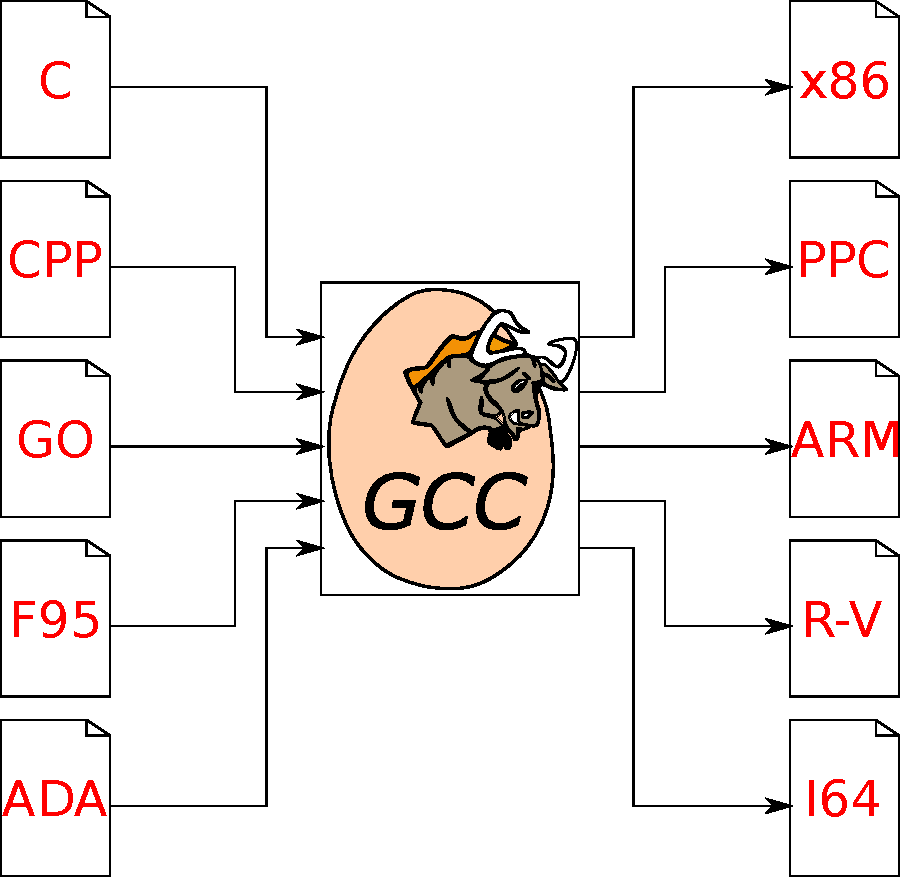
\includegraphics[scale=1.0]{logo.pdf}
    \par
}
\vspace*{\fill}
\normalsize{
\noindent\textcolor{darkgreen}{Giuliano Belinassi} \\
Timezone: GMT$-$3:00 \\
University of São Paulo -- Brazil \\
IRC: giulianob in \#gcc \\
Email: \href{mailto:giuliano.belinassi@usp.br}{\texttt{giuliano.belinassi@usp.br}} \\
Github: \url{https://github.com/giulianobelinassi/} \\
Date: \today
}
\newpage

\begin{section}{About Me}
    Computer Science Bachelor (University of São Paulo),
    currently pursuing a Masters Degree in Computer Science at the same
    institution. I've always been fascinated by topics such as
    High-Performance Computing and Code Optimization, having worked with
    a parallel implementation of a Boundary Elements Method software in GPU.
    I am currently conducting research on compiler parallelization and
    developing the \href{https://gcc.gnu.org/wiki/ParallelGcc}{ParallelGcc} project,
    having already presented it in \href{https://www.youtube.com/watch?v=jd6R3IK\_\_1Q}{GNU Cauldron 2019}.

    \textbf{Skills}: Strong knowledge in C, Concurrency, Shared Memory
    Parallelism, Multithreaded Debugging and other typical programming tools.
\end{section}

\begin{section}{Brief Introduction}

In \href{https://gcc.gnu.org/wiki/ParallelGcc}{ParallelGcc}, we showed that parallelizing the Intra Procedural optimizations
improves speed when compiling huge files by a factor of 1.8x in a 4 cores
    machine, and also showed that this takes 75\% of compilation time.

In this project we plan to use the LTO infrastructure to improve
compilation performance in the non-LTO case, with a tradeoff of generating
a binary as good as if LTO is disabled. Here, we will automatically detect
when a single file will benefit from parallelism, and procceed with the
compilation in parallel if so.

\begin{section}{Use of LTO}

The Link Time Optimization (LTO) is a compilation technique that allows the
compiler to analyse the program as a whole, instead of analysing and compiling
one file at time. Therefore, LTO is able to collect more information about
the program and generate a better optimization plan. LTO is divided in three
parts:

\begin{itemize}
    \item \emph{LGEN (Local Generation)}: Each file is translated to GIMPLE. This
        stage runs sequentially in each file and, therefore, in parallel in
        the project compilation.

    \item \emph{WPA (Whole Program Analysis)}: Run the Inter Procedural Analysis (IPA) in the
        entire program. This state runs serially in the project.

    \item \emph{LTRANS (Local Transformation)}: Execute all Intra Procedural Optimizations in
        each partition. This stage runs in parallel.
\end{itemize}

Since WPA can bottleneck the compilation because it runs serially in the entire
project, LTO was designed to produce faster binaries, not to produce binaries
fast.

Here, the proposed use of LTO to address this problem is to run the IPA
for each Translation Unit (TU), instead in the Whole Program, and automatically
detect when to partition the TU into multiple LTRANS to improve compilation performance.

The advantage of this approach is: by partitioning big files into multiple
partitions, we can improve the compilation performance by exposing these
partitions to the Jobserver. Therefore, it can improve CPU utilization in
manycore machines.  Generated code quality should be unaffected by this
procedure, which means that it should run as fast as when LTO is disabled.



\begin{itemize}

    \item It can generate binaries as good as when LTO is disabled.
    \item It is faster, as we can partition big files into multiple partitions
    and compile these partitions in parallel.
    \item It can interact with GNU Make Jobserver, improving CPU utilization.

\end{itemize}

\end{section}

\begin{section}{Planned Tasks}

I plan to use the GSoC time to develop the following topics:

\begin{itemize}
 \item{Week [1, 4] -- May 4 to May 27:} \\
  Update \texttt{cc1}, \texttt{cc1plus}, \texttt{f771}, \ldots, to partition
  the Compilation Unit (CU) after IPA analysis directly into multiple LTRANS
  partitions, instead of generating a temporary GIMPLE file, and to accept a
  additional parameter \texttt{-fsplit-outputs=<tempfile>}, in which the
  generated ASM filenames will be written to.

  There are two possible cases in which I could work on:
  \begin{enumerate}
    \item \textit{Fork}: After the CU is partitioned into multiple LTRANS, then
    \texttt{cc1} will fork and compile these partitions, each of them
    generating a ASM file, and write the generated asm name into
    \texttt{<tempfile>}.  Note that if the number of partitions is one, then
    this part is not necessary.

    \item \textit{Stream LTRANS IR}: After CU is partitionated into multiple
    LTRANS, then \texttt{cc1} will write these partitions into disk so that LTO
    can read these files and proceed as a standard LTO operation in order to
    generate a partially linked object file.
  \end{enumerate}

  1. Has the advantage of having less overhead than 2., as there is less IO operations,
  however it may be hard to implement as the assembler file may be already
  opened before forking, so caution is necessary to make sure that there are a
  1 - 1 relationship between assembler file and the compilation process. 2.
  on the other hand can easily interact with the GNU jobserver.

 \item{Week [5, 8] -- June 1 to June 26:} \\
  Update the \texttt{gcc} driver to take each file in \texttt{<tempfile>}, then
  assemble and partially link them together. Here, an important optimization is
  to use a named pipe in \texttt{<tempfile>} to avoid having to wait every
  partition to end its compilation before assembling the files.

 \item{Week 9 -- June 29 to July 3:} \textbf{First Evaluation} \\
  Deliver a non-optimized version of the project. Some programs ought to be
  compiled correctly, but probably there will be a huge overhead because so far
  there is no way of interacting with GNU Jobserver.

 \item{Week [10, 12] -- July 6 to July 24:} \\
  Work on GNU Make Jobserver integration. A way of doing this is to adapt
  the LTO WPA $\rightarrow$ LTRANS way of interacting with Jobserver. Another
  way is to make the forked \texttt{cc1} consume Jobserver tokens until the
  compilation finishes, then return the token when done.

 \item{Week 13 -- July 27 to 31:} \textbf{Second Evaluation} \\
  Deliver a more optimized version of the project. Here we should filter files
  that would compile fast from files that would require partitioning, and
  interact with GNU Jobserver. Therefore we should see some speedup.

\item{Week [14, 16] -- August 3 to 21:} \\
  Develop adequate tests coverage and address unexpected issues
  so that this feature can be merged to trunk for the next GCC
  release.

\item{Week 17: August 24 to 31} \textbf{Final evaluation}\\
  Deliver the final product as a series of patches for trunk.


\end{itemize}
\end{section}

\end{section}
\end{document}
